\documentclass[twoside,12pt,notitlepage]{Classes/CUEDthesisPSnPDF}

\defbibheading{bibliography}{\chapter{Bibliography}}
\bibliography{Dissertation/references}

\usepackage{appendix}
\usepackage{xcolor}
\usepackage{listings}
\usepackage{textcomp}

\usepackage{hyperref}
\usepackage{changepage}
\usepackage{etoolbox}

\usepackage{tikz}
\usetikzlibrary{shapes,arrows,positioning}

% Define block styles
\tikzstyle{decision} = [diamond, draw, %fill=blue!20,
    text width=4.5em, text badly centered, node distance=0.5cm, inner sep=0pt]
\tikzstyle{block} = [rectangle, draw, %fill=blue!20,
    text width=5em, text centered, rounded corners, minimum height=4em, node
    distance = 0.5cm]
\tikzstyle{block_spaced} = [rectangle, draw, %fill=blue!20,
    text width=5em, text centered, rounded corners, minimum height=4em, node
    distance = 1cm]
\tikzstyle{line} = [draw, -latex']
\tikzstyle{cloud} = [draw, ellipse, %fill=red!20,
    node distance=3cm, minimum height=2em]
\tikzstyle{decision answer}=[near start,color=black]


\raggedbottom                           % try to avoid widows and orphans
\sloppy
\clubpenalty1000%
\widowpenalty1000%

\addtolength{\oddsidemargin}{6mm}       % adjust margins
\addtolength{\evensidemargin}{-8mm}

\ifpdf
    \pdfinfo { /Title  (Docula - A Documentation Generation Engine)
               /Creator (TeX)
               /Producer (pdfTeX)
               /Author (Elliott Hillary <ejh67@cam.ac.uk>)
               /CreationDate (D:20121009000000)  %format D:YYYYMMDDhhmmss
               /ModDate (D:20121009000000)
               /Keywords (docula)}
    \pdfcatalog { /PageMode (/UseOutlines)
                  /OpenAction (fitbh)  }
\fi

% turn of those nasty overfull and underfull hboxes
\hbadness=10000
\hfuzz=50pt

% Comment out the next line to get single spacing
\onehalfspacing


\definecolor{solarized@base03}{HTML}{002B36}
\definecolor{solarized@base02}{HTML}{073642}
\definecolor{solarized@base01}{HTML}{586e75}
\definecolor{solarized@base00}{HTML}{657b83}
\definecolor{solarized@base0}{HTML}{839496}
\definecolor{solarized@base1}{HTML}{93a1a1}
\definecolor{solarized@base2}{HTML}{EEE8D5}
\definecolor{solarized@base3}{HTML}{FDF6E3}
\definecolor{solarized@yellow}{HTML}{B58900}
\definecolor{solarized@orange}{HTML}{CB4B16}
\definecolor{solarized@red}{HTML}{DC322F}
\definecolor{solarized@magenta}{HTML}{D33682}
\definecolor{solarized@violet}{HTML}{6C71C4}
\definecolor{solarized@blue}{HTML}{268BD2}
\definecolor{solarized@cyan}{HTML}{2AA198}
\definecolor{solarized@green}{HTML}{859900}

\lstdefinelanguage{treetop}[]{ruby}{
  morekeywords={rule},
  morecomment=[s]{<}{>}
}

\lstset{
    upquote=true,
    columns=fixed,
    tabsize=4,
    extendedchars=true,
    breaklines=true,
%    numbers=left,
    numbersep=5pt,
%    backgroundcolor=\color{solarized@base2},
    rulesepcolor=\color{solarized@base03},
    numberstyle=\tiny\color{solarized@base01},
    basicstyle=\footnotesize\ttfamily,
    keywordstyle=\color{solarized@green},
    stringstyle=\color{solarized@cyan}\ttfamily,
    identifierstyle=\color{solarized@blue},
    commentstyle=\color{solarized@base01},
    emphstyle=\color{solarized@red},
    showstringspaces=false
}

\lstnewenvironment{code}[1][]%
{
   \noindent
   \minipage{\linewidth}
   \vspace{0.5\baselineskip}
   \lstset{basicstyle=\ttfamily\footnotesize,#1}}
{\endminipage\vspace{0.5\baselineskip}}

\begin{document}

\pagestyle{empty}

\hfill{\LARGE \bf Elliott Hillary}

\vspace*{60mm}
\begin{center}
\Huge
{\bf Docula - A Documentation Generation Engine} \\
\vspace*{5mm}
Computer Science: Part II\\
\vspace*{5mm}
Girton College \\
\vspace*{5mm}
\today  % today's date
\end{center}

% set the number of sectioning levels that get number and appear in the contents
\setcounter{secnumdepth}{3}
\setcounter{tocdepth}{3}

\frontmatter % book mode only
\pagenumbering{roman}
\cleardoublepage
\chapter*{Proforma}

{\large
  \begin{tabular}{l l}
    Name:               & \bf Elliott Hillary                            \\
    College:            & \bf Girton College                             \\
    Project Title:      & \bf Docula - A Documentation Generation Engine \\
    Examination:        & \bf Computer Science - Part II, July 2013      \\
    Word Count:         & \bf \input{"dissertation.sum"}                 \\
    Project Originator: & Elliott Hillary                                \\
    Supervisor:         & Dr R.~Watts                                    \\
  \end{tabular}
}

\section*{Original Aims of the Project}
The intention of the project was to create software capable of producing
documentation from appropriately annotated source code. The software should be
compatible with existing comment formats and successfully output useful,
human-readable documentation.


\section*{Work Completed}
I successfully created a parser, and code capable of transforming the
resulting parse tree in to a set of HTML documents. The software created is also
capable of parsing directories of source code incrementally, so subsequent
executions complete much more quickly.

The parser produced does not have complete coverage of the C language, due
mainly to a lack of pre-processing being performed on the files being parsed, so
parsing of large codebases proved troublesome.


\section*{Special Difficulties}
Problems with tendonitis in the wrist caused some productivity problems
during Lent and Easter term.

\cleardoublepage
\chapter*{Declaration}

I, Elliott Hillary of Girton College, being a candidate for Part II of
the Computer Science Tripos, hereby declare that this dissertation and
the work described in it are my own work, unaided except as may be
specified below, and that the dissertation does not contain material
that has already been used to any substantial extent for a comparable
purpose. 

\bigskip
\leftline{Signed}

\medskip
\leftline{Date}


\tableofcontents

\mainmatter % book mode only
\pagestyle{fancy}
\pagenumbering{arabic}
% The Introduction should explain the principal motivation for the project.
% Show how the work fits into the broad area of surrounding Computer Science and
% give a brief survey of previous related work. It should generally be
% unnecessary to quote at length from technical papers or textbooks. If a simple
% bibliographic reference is insufficient, consign any lengthy quotation to an
% appendix.

\chapter{Introduction}
Whilst working on several large projects, I have noticed the difference good
documentation can make to the further development or maintenance of a code base.
Documentation can save hours of tedious work finding the areas of the source
code that require work, without even considering the benefits it also brings by
better informing the developer about the inner workings of the code itself. Good
documentation informs the reader of what a particular section of code does and,
depending on the situation, what design decisions were made and how the code
itself works. When written properly, documentation should inform the reader in
enough detail that they can begin using the code without having to dig into its
internals.

The problem with writing good documentation is that it requires developer time
\& skill to maintain, unfortunately most developers have neither. Documentation
generation helps to solve this problem, by minimising the amount of work a
developer has to do to produce documentation, meaning that they are more likely
to create useful documentation. First and foremost, documentation generation
allows for developers to write documentation in the source files themselves,
where it is later extracted by the generation software; this means that the
documentation is much more convenient to write, since it can be written
alongside the code. The additional benefit from this is that the generation
software can extract the information about the section being documented, such as
its type, and include this information in the documentation itself; this reduces
the amount of work the developer has to do, whilst also making it harder for the
documentation to become inconsistent with the code.

Software, such as doxygen\cite{website:doxygen} and
Javadoc\cite{website:javadoc}, already exists to perform these tasks and goes a
long way to making the lives of developers easier. These pieces of software, and
their alternatives, are widely used, but they offer an incomplete solution to
the problems they address; they focus on helping developers establish
\emph{what} a particular thing does, or is used for, but they do not try to
document the design decisions that led to this implementation nor the
considerations that drove them.

The intention of my project was to address these shortcomings.

% Principally, this chapter should describe the work which was undertaken before
% code was written, hardware built or theories worked on. It should show how the
% project proposal was further refined and clarified, so that the Implementation
% stage could go smoothly rather than by trial and error.

% Throughout this chapter and indeed the whole dissertation, it is essential to
% demonstrate that a proper professional approach was employed.

% The nature of this chapter will vary greatly from one dissertation to another
% but, underlining the professional approach, this chapter will very likely
% include a section headed “Requirements Analysis” and incorporate other
% references to the techniques of Software Engineering.

% The chapter will cite any new programming languages and systems which had to
% be learnt and will mention complicated theories or algorithms which required
% understanding.

\chapter{Preparation}
\section{Requirements}

\section{Comment Format}
In my proposal, I specifically mentioned the compatibility with existing comment
formats was highly important to produce a useful result; as such, consideration
about the format I was going to be using had to be undertaken before any work
could begin. Both doxygen and Javadoc's comment formats are similar to one
another, and together they have quite a large `market' share, so it was sensible
to design a format that was compatible with these as much as possible. Ideally,
my format should be equal to or a superset of their formats, so that any
comments written with them in mind will work with the software I write.

With that in mind, I designed a format along the following lines (a full version
of which can be found in the appendix):

\begin{lstlisting}[language=c, escapechar=~]
  /**
   * Summary
   *
   * Full Description
   *
   * ~{\color{solarized@cyan} @param[in, out]}~ ptr Description of parameter ptr
   * ~{\color{solarized@cyan} @param[in]}~ size Description of parameter size
   * ~{\color{solarized@cyan} @return}~ Description of return value.
   */
  void *realloc(void *ptr, unsigned int size);
\end{lstlisting}

\begin{itemize}
  \item The first paragraph (i.e.~up to the first empty line) is considered to
    be a summary, and gives a brief outline of the intended use. This is
    standard practice with Javadoc, and can be enabled in doxygen.
  \item The following paragraphs make up the full description, expanding on the
    summary, describing in more detail what it does and how it should be used.
  \item @-annotations
    \begin{itemize}
      \item \lstinline|@param| annotations are used to describe the individual
        parameters and their purpose.
      \item The square-bracket suffixes to \lstinline|@param| annotations are
        for describing the flow of data, that is whether the variable is only
        used for input, output or both. These are described as \lstinline|[in]|,
        \lstinline|[out]| \& \lstinline|[in,out]| respectively. If a parameter
        is absent a flow annotation, it will be assumed that it is
        \lstinline|[in]|.
        doxygen already uses this way of describing flows; Javadoc does not have
        any such feature, this is presumably because Java only does
        pass-by-value and so this was deemed unnecessary.
      \item \lstinline|@return| is used to describe what will be returned by the
        function; this may include under what conditions it will return an error
        and what those error values may be.
    \end{itemize}
    \item Summary \& Description sections can be applied to things other than
      functions, the @-annotations cannot, as they would be meaningless.
\end{itemize}

\section{Tools}
  \subsection{Programming Language}
    I opted to use Ruby to implement this project, whilst I do not have as much
    experience with Ruby as some other languages (like Java), I felt it was best
    suited to the project. This is because one of Ruby's strengths is in its
    powerful text-manipulation capabilities, whereas processing Strings in Java
    can be quite heavyweight in terms of memory.

    Additionally, having looked into implementing parsers in various languages,
    I found that Treetop\cite{website:treetop} was particularly to my liking.
    Treetop is a domain-specific language for Ruby, that facilitates the
    creation of parsing expression grammars; one of the particularly useful
    things about Treetop is that it allows you to define specific types for
    matched rules to instantiate, so that a lot of the effort of having to walk
    a parse tree can be alleviated. This will be discussed in further detail in
    the Implementation chapter.

    I was already partially familiar with Ruby, however I made use of
    \emph{Eloquent Ruby}\cite{book:eloquent_ruby} to further hone my knowledge
    of the language.

% This chapter should describe what was actually produced: the programs which
% were written, the hardware which was built or the theory which was developed.
% Any design strategies that looked ahead to the testing stage might profitably
% be referred to (the professional approach again).

% Descriptions of programs may include fragments of high-level code but large
% chunks of code are usually best left to appendices or omitted altogether.
% Analogous advice applies to circuit diagrams.

% Draw attention to the parts of the work which are not your own. Making
% effective use of powerful tools and pre-existing code is often laudable, and
% will count to your credit if properly reported.

% It should not be necessary to give a day-by-day account of the progress of the
% work but major milestones may sometimes be highlighted with advantage.

\chapter{Implementation}

\section{The Parser}
To implement my parser, I made use of an existing domain-specific language
available as a Ruby library called Treetop\cite{website:treetop}; Treetop allows
for easy implementation of Parsing Expression Grammars, which, simply put, are
grammars that built up out of a combination of rules and regular expressions.

Parsing Expression Grammars were particularly appealing to me for two reasons:
firstly, they are essentially a more powerful version of regular expressions,
with which I am already familiar and secondly, they can be made to run in
constant time if implemented as a packrat parser, which Treetop does. This
constant time guarantee is provided by the process of memoization, which trades
off time for space by caching previous inputs and the resulting parse trees to
remove the need for repeated computations.

Treetop grammars are written as their own .treetop files, which are then used
to generate the parsers by the \lstinline|tt| program. The end result is a Ruby
source file which can be included and used to parse the language defined by the
grammar. Treetop also allows you to define a class that nodes within the parsed
data should be instantiated as, this means that nodes can be given methods with
which they can parse themselves or their children; which is much preferable to
the traditional methods of writing code to walk the tree structures.

\begin{code}[language=treetop]
  rule comment
    '//' ( !EOL .)* EOL <CommentNode>
    / '# ' ( !EOL .)* EOL <CommentNode>
    / (multiline_comment) <CommentNode>
  end
  rule multiline_comment
    '/*'
    (
      !'*/'
      (. / EOL)
    )*
    '*/'
  end
  rule EOL
    [\n]
  end
\end{code}

Above is a snippet from my Treetop grammar for C, defining the grammar for
comments. The rule \lstinline|comment| contains an ordered choice of expressions
that define each type of comment available in C, and informs Treetop that they
should be instantiated using the class \lstinline|CommentNode|;
\lstinline|CommentNode| defines a method with which the text of the comment
can be extracted.


  \subsection{Regression Testing}
    To ensure that I was properly implementing my grammar for C, I wrote some
    tests for my parser that would check that parsing a particular piece of code
    would yield a valid result. This was the quickest \& easiest way of building
    up a working grammar for the language and allowed me to be confident that
    what I had written would function correctly as I moved forward.

    This was implemented using \lstinline|TestCase|, a class that is part of the
    Ruby standard library, and simply involves defining methods that execute the
    code required for each test and uses various types of assertions to ensure
    that the results are as expected.

    The process went as follows:

    \begin{center}
    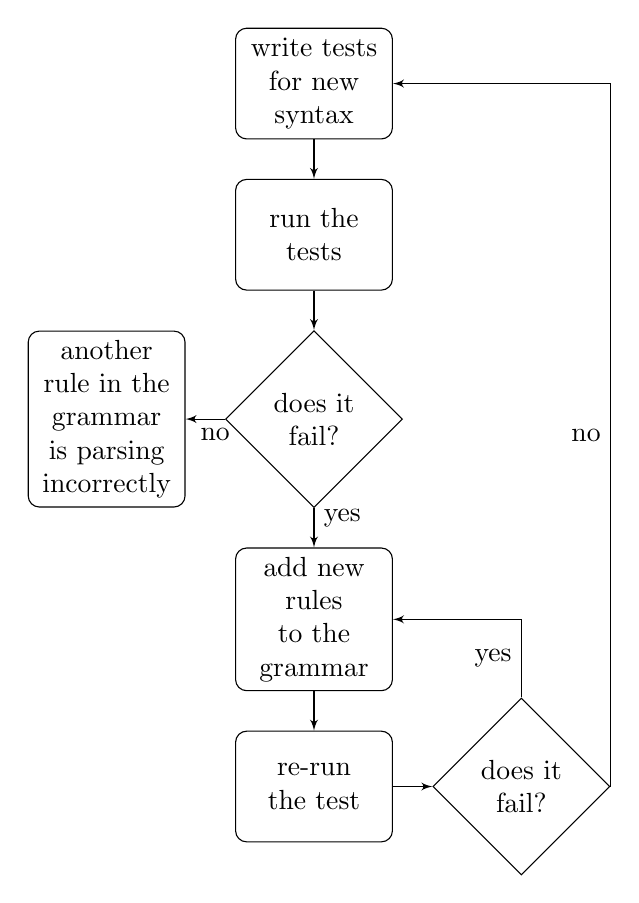
\begin{tikzpicture}[node distance = 2cm, auto]
        % Place nodes
        \node [block] (init) {write tests for new syntax};
        \node [block, below=of init] (run) {run the tests};
        \node [decision, below=of run] (fail) {does it fail?};
        \node [block, left=of fail] (debug) {another rule in the grammar is
          parsing incorrectly};
        \node [block, below=of fail, node distance=3cm] (develop) {add new rules
          to the grammar};
        \node [block, below=of develop, node distance=3cm] (rerun) {re-run the
          test};
        \node [decision, right=of rerun] (refail) {does it fail?};
        % Draw edges
        \path [line] (init) -- (run);
        \path [line] (run) -- (fail);
        \path [line] (fail) -- node[decision answer] {no} (debug);
        \path [line] (fail) -- node[decision answer] {yes} (develop);
        \path [line] (develop) -- (rerun);
        \path [line] (rerun) -- (refail);
        \path [line] (refail.east) |- node[decision answer] {no} (init);
        \path [line] (refail) |- node[decision answer] {yes} (develop);
    \end{tikzpicture}
    \end{center}

  \subsection{Parsing Problems}
    As I wrote my initial grammar for the C parser, it became apparent that I
    was having some problems; I got to the point where implementing new rules
    within the grammar would cause other tests to fail, the problem was that
    describing C correctly required such a huge grammar that the rules were
    interacting in ways I had not accounted for. This meant that progress on the
    grammar slowed to a crawl, and it became apparent that the grammar would
    need to be largely rethought to fully parse C.

    I realised, however, that in order to parse C for the purposes of generating
    documentation, I did not need my parser to completely understand the
    language, instead it needed to only understand enough to parse to top level.
    I therefore wrote a new, simpler parser that understood how to navigate
    through the C files, rather than parsing all of it; this brought an added
    advantage of improving the runtime of the parser.

    Instead of parsing function bodies, the simplified parser contains rules to
    match pairs of braces within functions, ignoring those in strings and
    comments, to understand where functions begin \& end. With global variable
    assignments, the parser has rules to match from an equals sign to the
    semicolon at the end of the line. These simplifications allowed for me to
    dispense with the expensive and complicated parsing of control structures
    and arithmetic, and reduced the grammar from ${\sim}$500 lines in the
    original (unfinished) grammar to ${\sim}$300 lines for the completed
    simplified one.

    Ideally, some or all of the more complex behaviour would be restored to the
    grammar, as it would allow for better analysis of the parsed language, such
    as including in the documentation what was referenced by a particular
    function. Given the time constraints involved in the project, this could not
    be performed.

\section{Handling the Data}
After the source files have been parsed into a parse tree, the useful data can
be extracted; using the methods that were added into the parse tree by Treetop,
the code runs through the functions, variables \& other pieces of data and pulls
out the needed information to be stored in the database.

To store the data I opted to use SQLite, as it requires no configuration to use
and stores all data in a file, rather than on a SQL server; this means that no
setup of databases is required on the part of the user. I used the
sqlite3\cite{website:sqlite} Ruby library to interact with my database, which
allows you to interact with data from the database using the normal Ruby types.

  \subsection{Processing}
    The classes I defined for use in the parse tree provide easy access to the
    data within the nodes, and their subtrees, whilst masking the specifics of
    the tree itself; this means that future additions to the parser and the way
    in which it works will not affect the processing of the data. In addition,
    this allows for the reuse of the processing code on the parse trees of
    different languages, provided that the nodes in that tree expose the same
    methods.

    Since some functions in the source being parsed may only be partially
    documented, I needed to account for this in my code to ensure that the
    resulting data was consistent; in particular, if a function is documented
    the hash containing information about the prototype will contain extra
    information. Uniting the arguments with their documentation proved
    interesting, and I had to write the code for managing it several times
    before I created a solution that provided an appropriate output regardless
    of input.

    \begin{code}[language=ruby, gobble=6]
      if function.documented?
        prototype[:arguments] = prototype[:arguments].zip(prototype[:params]).map do |a,d|
          d ? a.merge(d) : a
        end
        prototype.delete(:params)
      end
    \end{code}

    This small section of code was the eventual solution, and in just a few
    lines accomplishes quite a bit. The array containing the arguments
    parsed, from the function prototype itself, is merged with the array
    containing the documentation for each argument, producing a new array. This
    array is contains several arrays, each holding the documentation and
    prototype for one argument; finally, the map function returns the array I
    need by merging the two hashes together, if the argument is documented, or
    returning the just the argument's hash if no documentation exists. The
    example data below demonstrates the process.

    \begin{code}[language=ruby, gobble=6]
      A = [{a => 1}, {b => 2}, {c => 3}]
      B = [{d => 4}, {}, {f => 6}]

      # After zipping A & B...

      C = [[{a => 1}, {d => 4}], [{b => 2}], [{c => 3}, {f => 6}]]

      # After mapping C...

      D = [{a => 1, d => 4}, {b => 2}, {c => 3, f => 6}]
    \end{code}

      \subsubsection{Post-processing}
        Once the data for all files in the directory has been added to the
        database, some extra processing takes place to resolve which files
        include one another. By looping through all the includes encountered
        and determining whether it refers another file that has been processed,
        links are built between files, which are later used by the output stage
        to allow a user to jump from one file to one of its includes easily.

        To determine if one file refers to another, I decided to check whether a
        following the path described in the include exists, relative to that
        file. This is by no means a fool-proof solution, as it does not take
        into account the include paths passed to a compiler, but the only other
        sensible solution to this problem would be to also parse the Makefile
        (or similar file in another build system) to extract the include paths
        used. Given the number of different build systems used and the time
        taken to implement another grammar for parsing any of them, I concluded
        that this was not a valid solution in the time available.

  \subsection{Storage}


    \subsubsection{Foreign Keys}

\section{Generating the Output}

Once all the data has been processed and stored, the output can be generated;
currently there is only one available output format, HTML, however the
outputting process has been designed so that a new output format can be easily
added. To do this, a generic \lstinline|Output| class was created that defines
methods that can be used to extract all the data required for producing the
output. This means that creation of a new output format only requires the
definition of a new subclass of \lstinline|Output| that defines an
\lstinline|output| method, which can call the other methods already defined to
get its data.

Generating output can be a messy process, especially with HTML, as inevitably
code and HTML markup end up being interleaved together; I have done my best to
separate the two out by defining functions that produce particular sections of
commonly repeated HTML, such as creating links and table rows, to increase the
readability of the code, however there is only so much this can be done.

\begin{code}[language=ruby, gobble=2]
  def row_with_id(id, *entries)
    if entries == []
      "<tr id=\"#{id}\"></tr>"
    else
      "<tr id=\"#{id}\"><td>#{entries.join("</td><td>")}</td></tr>\n"
    end
  end
\end{code}

The function above allows me to create a new row in a table
\lstinline|row_with_id("some_id", ["item1", "item2"])| when I need one, rather
than repeating the same HTML over \& over. String interpolation also helps the
situation greatly, as it allowed me to write much more concise code; the above
code without it would have been much more verbose and complicated, line 5 would
have been:

\begin{code}[language=ruby, gobble=2]
  "<tr id=\"" << id.to_s << "\"><td>" << entries.join("</td><td>") << "</td></tr>\n"
\end{code}

This would have also been more expensive to compute, as it requires mutating the
string four times, rather than just creating it correctly in the first place.
This is one example of a reason I chose Ruby in the in my proposal.

  \subsection{Linking Between Files}
    Linking between the outputted pages, for things like the list of includes,
    was solved using \lstinline|Pathname|, another class available in the Ruby
    standard library. \lstinline|Pathname| allows you to determine the relative
    path between two files; since I had ensured that the directory structure of
    my outputted data matched that of the input data, the relative path between
    the two source files is also the relative path between the HTML files. This
    meant that producing these paths was fairly easy.

    Taking this a step further, I also implemented linking a type to the file it
    was originally declared in; this was done with \lstinline|Pathname| as
    above, and a \lstinline|type| method in \lstinline|Output| that looks up
    types in the SQLite database.

    \begin{code}[language=sql, gobble=6]
      SELECT types.*, files.path FROM
       (SELECT id, file_id, name, 'typedef' FROM typedefs WHERE typedefs.name = ?
        UNION ALL
        SELECT id, file_id, name, 'define' FROM defines WHERE defines.name = ?
       ) AS 'types' INNER JOIN files ON types.file_id = files.id
    \end{code}

    This SQL statement looks up a type in the \lstinline|typedef| \&
    \lstinline|define| tables, unioning the two result sets together to ensure
    that we get results from either, and then performs an inner join of these
    results against the files table to get the information on the file that the
    typedef or define was found in. This results in a rather large SQL
    statement, which can be a little complicated to understand, however it is
    much quicker than running three queries and producing the result in Ruby.

\section{The Command-Line Interface}
The command line interface ties all of the previous stages together, allowing
for everything to be used together conveniently without requiring any Ruby
knowledge on the part of the user.

Aside from making the process more convenient, the command line interface also
provides easy manipulation of the options the program uses and performs the
cleaning and the initial setup of the database.

Within this same section of code is also where the traversal of directories to
find the files to be parsed takes place; Ruby's use of blocks allows the code
for this to be written quickly and clearly. I wrote a small method,
\lstinline|recurse|, that recurses down through the directories contained within
a particular path, and yields the files contained in them back to its caller.
This way of doing this made working through the files as convenient as working
through the elements of an array, without having to store all of the filenames
in an array first.

% \begin{lstlisting}[language=ruby, gobble=2]
%   # Compare:

%   ["test.h", "test.c", "another_file.txt"].each do |element|
%     if parsers[File.extname(element)]
%       # ...
%     end
%   end

%   # versus

%   Dir.recurse(options[:directory]) do |file|
%     if parsers[File.extname(file)]
%       # ...
%     end
%   end
% \end{lstlisting}

The process goes as follows:

\begin{center}
    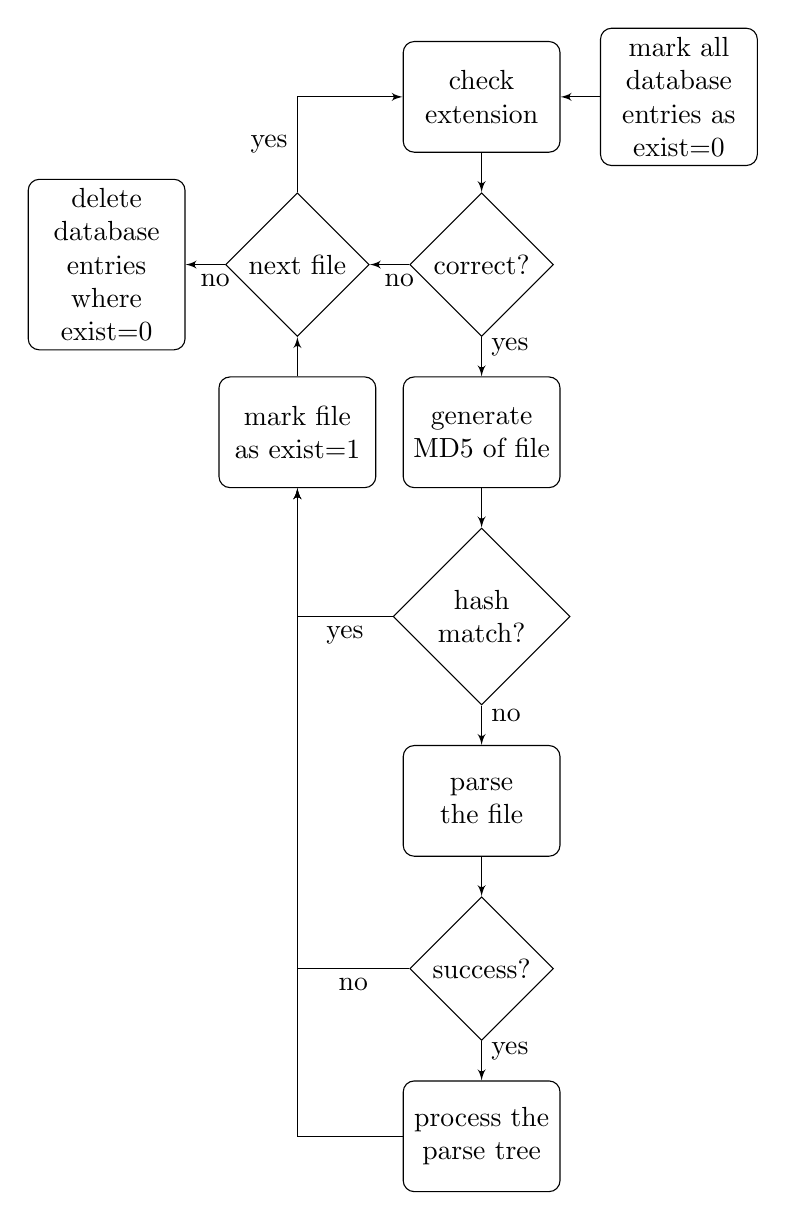
\begin{tikzpicture}[node distance = 0.5cm, auto]
        % Place nodes
        \node [block] (exist) {mark all database entries as exist=0};
        \node [block, left=of exist] (check) {check extension};
        \node [decision, below=of check] (extension) {correct?};
        \node [decision, left=of extension] (next) {next file};
        \node [block, below=of extension] (md5) {generate MD5 of file};
        \node [decision, below=of md5] (match) {hash match?};
        \node [block, below=of next] (mark) {mark file as exist=1};
        \node [block, below=of match] (parse) {parse the file};
        \node [decision, below=of parse] (success) {success?};
        \node [block, below=of success] (process) {process the parse tree};
        \node [block, left=of next] (delete) {delete database entries where
          exist=0};
        % Draw edges
        \path [line] (exist) -- (check);
        \path [line] (check) -- (extension);
        \path [line] (extension) -- node[decision answer] {yes} (md5);
        \path [line] (extension) -- node[decision answer] {no} (next);
        \path [line] (md5) -- (match);
        \path [line] (match) -| node[decision answer] {yes} (mark);
        \path [line] (match) -- node[decision answer] {no} (parse);
        \path [line] (parse) -- (success);
        \path [line] (success) -| node[decision answer] {no} (mark);
        \path [line] (success) -- node[decision answer] {yes} (process);
        \path [line] (mark) -- (next);
        \path [line] (process) -| (mark);
        \path [line] (next) |- node[decision answer] {yes} (check);
        \path [line] (next) -- node[decision answer] {no} (delete);
    \end{tikzpicture}
    \end{center}

  \subsection{Option Parsing}
    Ruby has an extremely robust command-line option parser built into the
    standard library, so there was no need to roll my own or make use of an
    external library. \lstinline|OptionParser| made defining options simple, and
    produces help text automatically, so the whole process was quite straight
    forward.

    The following snippet is sufficient to describe a verbose option for a
    program:

    \begin{lstlisting}[language=ruby,gobble=6]
      options = {}
      OptionParser.new do |opts|
        opts.banner = "Usage: example.rb [options]"

        opts.on("-v", "--[no-]verbose", "Run verbosely") do |v|
          options[:verbose] = v
        end
      end.parse!
    \end{lstlisting}

    Using \lstinline|OptionParser| allowed me to specify default options within
    my \lstinline|options| hash, which can then be overridden by the user on the
    command-line.

    \lstinline|OptionParser| also allows you to define an option that takes only
    certain inputs, using this it was easy to create and option for choosing the
    output format; even though there is only one currently, this project was
    designed with extensibility in mind.

    \begin{code}[language=ruby, gobble=6]
      o.on("--format FORMAT", outputs, "Select output format",
           "  (#{outputs.keys.join(", ")})") do |format|
        options[:format] = format
      end
    \end{code}

    This adds an option that will accept any entry that is a key in the
    \lstinline|outputs| hash, and sets the appropriate entry in the
    \lstinline|options| hash to the value of the entry, which is the output
    class to use. This means that adding a new output format requires only a
    subclass of \lstinline|Output| and an entry referencing it in the
    \lstinline|outputs| hash.

\chapter{Evaluation}

% This chapter is likely to be very short and it may well refer back to the
% Introduction. It might properly explain how you would have planned the project
% if starting again with the benefit of hindsight.

\chapter{Conclusion}
I have successfully produced software capable of transforming source code, using
appropriately-styled comments, into human-readable documentation. The software
does not completely parse the C language correctly, mainly due to difficulties
in parsing preprocessor macros; given more time, this should be fairly easy to
fix. As the results in the previous chapter show, the software parses source
trees faster on subsequent runs than doxygen, due to the use of persistent
storage.

Whilst the software I have produced does indeed produce documentation, it does
not address the shortcomings that I identified in existing documentation
generation software, namely that they do not allow the developer to fully
describe ``the design decisions that led to this implementation nor the
considerations that drove them''. Due in part to time constraints, difficulties
and hold-ups in the implementation process, the software I have produced only
goes as far as existing software does in displaying documentation, however I
believe that I have designed my system in a modular enough way that these things
could be added in the future without any significant re-designs taking place.

I originally opted to use Treetop for creating the parser because it allowed me
to implement it in a way that was logical and familiar to me, with hindsight, it
would perhaps have been better (at least, in the time that was available to me)
to make use of an infrastructure such as LLVM\cite{website:llvm} to facilitate
the parsing. This would have also given me the added advantage of being able to
perform some static analysis on the code, potentially allowing for the generated
documentation to display information about the usage of functions. The downside
to this is that LLVM would only be usable with languages that have a front-end
implemented for it, whereas Treetop could be used to parse any language. With
hindsight, I would have at least considered using LLVM instead of, or in
combination with, Treetop to do my parsing.

Overall I believe that my project was a modest success, despite not doing
everything I set out to do, it does go a long way to being a competent
documentation generator.


\printbibliography

\begin{appendices}
\chapter{Comment Format}

\begin{lstlisting}[language=c]
    /**
     * In order to ensure compatibility with Doxygen, I needed to create a
     * comment format that was as similar to theirs as possible.
     * Any block comment with a double star opening will be considered for a
     * documentation string.
     */

     /// Triple slashes opening a single line comment are also considered.

     /**
      * Documentation immediately preceding a function definition will become
      * associated with that function.
      *
      * Typically, the first paragraph is a summary, with the subsequent
      * paragraphs providing greater detail; this can be disabled in the
      * options.
      *
      * @param[in] Description of first argument
      * @param[inout] Description of second argument
      * @return Description of return value
      * @error Describes what make be returned in the case of an error.
      *
      * The @param annotations are for describing the arguments passed into
      * the function - what they represent and/or the range or valid values -
      * they also specify whether the argument is used solely for input,
      * output, or both ([in], [out] and [inout], respectively).
      */
    int example(int arg1, char* arg2);

    /// Documentation may also precede variables...
    int important_var;

    /// ... Or even #defines.
    #define ULTIMATE_ANSWER 42

    /**
     * @file
     *
     * Documentation marked with the @file annotation denote that they are
     * referring to the file as a whole.
     *
     * These comments may also include other relevant information, such as:
     * @copyright My Company Inc.
     * @author Elliott Hillary
     * @created 2012-10-18
     */
\end{lstlisting}

\chapter{Questionnaire}

\hypersetup{
  linkcolor=black,
  linkbordercolor={0 0 0},
  colorlinks=false
}

\def\LayoutTextField#1#2{\makebox[6em][l]{#1}\raisebox{-.5ex}{#2}}
\def\LayoutChoiceField#1#2{\makebox[6em][l]{#1}#2}
\newdimen\longline
\longline=\textwidth\advance\longline-6em

\makeatletter
\patchcmd{\HyField@FlagsRadioButton}{\HyField@SetFlag{Ff}{Radio}}{}{}{}
\makeatother
\def\DefaultOptionsofRadio{print}

  \begin{center}
    \bf Docula: Evaluation Questionnaire
  \end{center}
  Along with this questionnaire you should have received a .gem file; to allow
  for convenient use of docula whilst testing it functionality, please execute
  the following in a shell\footnote{Depending on your Ruby setup, this may need
  to be executed as root}:
  \begin{verbatim}
    $ gem install --local docula-*.gem
  \end{verbatim}
  This will properly install docula and its dependencies onto your system. You
  should then be able to use the \verb|docula| command to generate documentation
  for a particular directory. The resulting documentation should be available in
  the \verb|output/| directory by default.

  When testing has completed, you can remove docula with:
  \begin{verbatim}
    $ gem uninstall docula
    $ gem cleanup
  \end{verbatim}
  The second command will remove all the dependencies that were installed,
  provided they are no longer required, leaving your system as it was before
  testing.

  To remove any traces of docula from a directory you used it in, simply:
  \begin{verbatim}
    $ rm -rf .docula/ output/
  \end{verbatim}

  The rest of this document contains some questions that will help me to
  evaluate the functionality of \verb|docula|, please take the time to fill them
  out; all non-multiple choice questions are optional.

  \newpage

  \begin{Form}
    \noindent
    Were you able to install the software using the instructions on the previous
    page?
    \medskip
    \begin{center}
      \ChoiceMenu[radio,name=install]{}{Yes, No}\\
    \end{center}

    \bigskip
    \noindent
    \verb|docula| can generate documentation for C source \& header files, if
    you were to run it on a directory containing these files, it should produce
    documentation.\\
    Were you able to generate successfully generate any documentation?
    \medskip
    \begin{center}
      \ChoiceMenu[radio,name=generate]{}{Yes, No}\\
    \end{center}

    \bigskip
    \noindent
    When running \verb|docula|, did any of your source files fail to be parsed?
    If so, how many?
    \medskip
    \begin{center}
      \ChoiceMenu[radio,name=generate]{}{None, A Few, A Lot, Most, All}\\
    \end{center}

    \bigskip
    \noindent
    How did the speed compare to your usual documentation generation software?
    \medskip
    \begin{adjustwidth}{-2cm}{-2cm}
    \begin{center}
      \medskip
      \ChoiceMenu[radio,name=speed]{}{Much Slower, Slower, About the Same,
      Quicker, Much Quicker}\\
      \bigskip
    \end{center}
    \end{adjustwidth}

    \bigskip
    \noindent
    \verb|docula| uses the checksums of files to determine whether documentation
    needs to be regenerated when it is rerun. If you make a change to one or
    two files in your directory, \verb|docula| should only need to re-parse
    those files.\\
    How did the speed compare to your usual documentation generation software on
    the second execution?
    \medskip
    \begin{adjustwidth}{-2cm}{-2cm}
    \begin{center}
      \medskip
      \ChoiceMenu[radio,name=speed2]{}{Much Slower, Slower, About the Same,
      Quicker, Much Quicker}\\
      \bigskip
    \end{center}
    \end{adjustwidth}

    \bigskip
    \noindent
    How does the documentation produce compare with your usual documentation
    generation software?
    \medskip
    \begin{adjustwidth}{-2cm}{-2cm}
    \begin{center}
      \medskip
      \ChoiceMenu[radio,name=doccompare]{}{Much Better, Better, About the Same,
      Worse, Much Worse}\\
    \end{center}
    \end{adjustwidth}
    \medskip
    Why?\\
    \medskip
    \TextField[name=doccomment,multiline=true,width=\longline,height=2in,
      borderwidth=0,backgroundcolor={.85 .85 .85}]{}\\

    \bigskip
    \noindent
    Was there anything in particular that you felt was missing from the
    documentation?\\
    \medskip
    \TextField[name=missingcomment,multiline=true,width=\longline,height=2in,
      borderwidth=0,backgroundcolor={.85 .85 .85}]{}\\

    \bigskip
    \noindent
    Additional Comments\\
    \medskip
    \TextField[name=additionalcomment,multiline=true,width=\longline,height=2in,
      borderwidth=0,backgroundcolor={.85 .85 .85}]{}\\
  \end{Form}

  \begin{center}
    \bigskip\hrule\bigskip
    \emph{Thank you for taking the time to complete this questionnaire.}
  \end{center}

\chapter{Project Proposal}
% Draft #1 (final?)

% Main document

\section*{Introduction, The Problem To Be Addressed}


Many students write their CST dissertations in \LaTeX\ and
spend a fair amount of time learning just how to do that. The purpose of 
this project is to write a demonstration dissertation that explains in
detail how it done.  

This core proposal document will be augmented by a separately-printed
cover sheet at the front and a resource form at the end.  Additional
sheets for risk assessment and human resources may also need to be included.

This document will repeat much of the material that is summarised on the additional sheets.

\section*{Starting Point}

{\em Describe existing state of the art, previous work in this area, libraries and databases to be used.
Describe the state of any existing codebase that is to be built on.  }

I am already able to write prose using the English language. I have an online dictionary. etc..

\section*{Resources Required}

{\em A note of the resources required and confirmation of access.}

For this project I shall mainly use my own quad-core computer that runs Fedora Linux. Backup
will be to github and/or to an SVN repository on an external hard disk that is dumped to writable CD/DVD media.
I have another similar computer to hand should my main machine suddenly fail.
I require no other special resources.

\section*{Work to be done}

{\em Describe the technical work.}

The project breaks down into the following sub-projects:

\begin{enumerate}

\item The construction of a skeleton dissertation with the required 
structure. This involves writing the Makefile and makeing dummy files
for the title page, the proforma, chapters 1 to 5, the appendices and
the proposal.

\item Filling in the details required in the cover page and proforma.

\item Writing the contents of chapters 1 to 5, including examples
of common \LaTeX\ constructs.

\item Adding a example of how to use floating figures and encapsulated
postscript diagrams.

\end{enumerate}

\section*{Success Criterion for the Main Result}


The project will be a success if I have a completed dissertation with the correct chapter
titles and I have achieved my other success criterion, which is to blah ...



\section*{Possible Extensions}

{\em Potential further envisaged evaluation metrics or extensions.}

If I achieve my main result early I shall try the following alternative experiment or method of evaluation ...


\section*{Timetable: Workplan and Milestones to be achieved.}


{\em Perhaps list ten or so  two-week work-packages.}

Planned starting date is 16/10/2011.

\begin{enumerate}

\item {\bf Michaelmas weeks 2-4} Learn to use X. Read book Y. Read papers Z.

\item {\bf Michaelmas weeks 5-6} Do preliminary test of Q.

\item {\bf Michaelmas weeks 7-8} Start implementation of main task A.

\item {\bf Michaelmas vacation} Finish A and start main task B.

\item {\bf Lent weeks 0-2} Write progress report. Generate corpus of test examples. Finish task B.  

\item {\bf Lent weeks 3-5} Run main experiments and achieve working project.

\item {\bf Lent weeks 6-8} Second main deliverable here.

\item {\bf Easter vacation:} Extensions and writing dissertation main chapters.

\item {\bf Easter term 0-2:}  Further evaluation and complete dissertation.

\item {\bf Easter term 3:} Proof reading and then an early submission so as to concentrate on examination revision.

\end{enumerate}


 


\end{appendices}

\end{document}
